\section{Formulare}

Formulare sind ein ständiger Begleiter in unserem Leben – von der Geburt bis zum Tod sind sie in Form von Rechnungen, Bestellungen, Wohngeldanträgen, Eheschließungsunterlagen, Krankenscheinen etc. präsent. Ihre Geschichte reicht bis ins Jahr 1450 zurück, beginnend mit einem Ablassbrief \citep{formulare_schwesinger_2007}. Im Laufe der Zeit haben sich Formulare in ihrer Gestaltung immer wieder gewandelt. Heute verleihen zwei Schlüsselbegriffe den Formularen eine neue Dimension: eCommerce und eGovernment. Diese Konzepte haben Formulare ins Internet gebracht und sie damit in die digitale Welt überführt. Unabhängig von ihrer physischen oder digitalen Form, hat Dirk Baecker \citep[S. ~3]{plener_formular_2021} eine Definition für Formulare erfasst: ``Formulare sind von einer Ordnung bereitgestellte und im Rahmen dieser Ordnung verwaltete Texte mit Lücken, die von individuellen Fällen ausgefüllt werden, die von dieser Ordnung gesucht werden oder diese Ordnung in Anspruch nehmen'' \\

Diese historische Entwicklung von Formularen unterstreicht ihre anhaltende Bedeutung in unserem Leben. Die Definition von Baecker hebt hervor, dass Formulare nicht nur einfache Dokumente sind, sondern vielmehr strukturierte Instrumente, die es ermöglichen Informationen zu erfassen und zu verarbeiten und den NutzerInnen auch in modernen Formaten zur Verfügung zu stellen.\\

Die Entwicklung hin zu eCommerce und eGovernment, leitet uns zu einem zentralen Aspekt der modernen Verwaltung über: der Digitalisierung und Bereitstellung von kundenorientierten digitalen Formularen. Diese Transformation spielt eine entscheidende Rolle in der Art und Weise, wie NutzerInnen mit der Verwaltung interagieren und Dienstleistungen in Anspruch nehmen.\\

Mit dem Prozess der Digitalisierung werden immer mehr Online-Formulare entwickelt und zur Verfügung gestellt. Dies bietet Bequemlichkeit des Ausfüllen via Internet. Online-Formulare können die Eingaben automatisch ergänzen, überprüfen und auswerten. Dies führt zu einer höheren Effizienz, Fehlervermeidung, kürzeren Bearbeitungszeiten und verbesserten Nachverfolgung. Zudem sind sie umweltfreundlicher. Insgesamt erleichtern sie die Kommunikation erheblich und verbessern den Zugang zu angebotenen Dienstleistungen.\\


\cite{formulare_schwesinger_2007} hat in seinem Buch einer eingehenden Prüfung unterzogen und dabei die folgenden Vorzüge digitaler Formulare herausgefiltert:
\begin{itemize}
    \item sie sind nichtlinear: eingebettete Links erlauben den NutzerInnen von Frage zu Frage springen und nur relevante Abschnitte werden für Nutzerinnen eingeblendet.
    \item sie validieren Eingaben: ob es sich um eine Zahleneingabe oder um die Auswahl aus vorgegebenen Antworten und Pflichtfelder handelt, werden die Eingaben zeitgleich überprüft.
    \item sie helfen beim Ausfüllen: zu jedem Eingabefeld sind Hilfetools, Hinweise oder automatische Vervollständigungsfunktionen sichtbar integriert.
    \item sie können rechnen: die komplexe Rechenalgorithmen stecken dahinter, um sofortige Ergebnisse anzuzeigen.
    \item sie können barrierefrei sein: Schrift zu vergrößen, Farben anzupassen oder Texte vorzulesen ist sogar in der öffentlichen Verwaltung gesetzlich vorgeschrieben
    \item sie sind leichter zu aktualisieren: digitale Formulare beim Abruf sind aktuell. Dafür müssen die Formulare an einer Stelle zentral geändert werden.
    \item sie sind schneller: sofort, jederzeit an beliebigen Empfängern übertragbar sind.
\end{itemize}


\begin{figure}[ht]
  \centering
  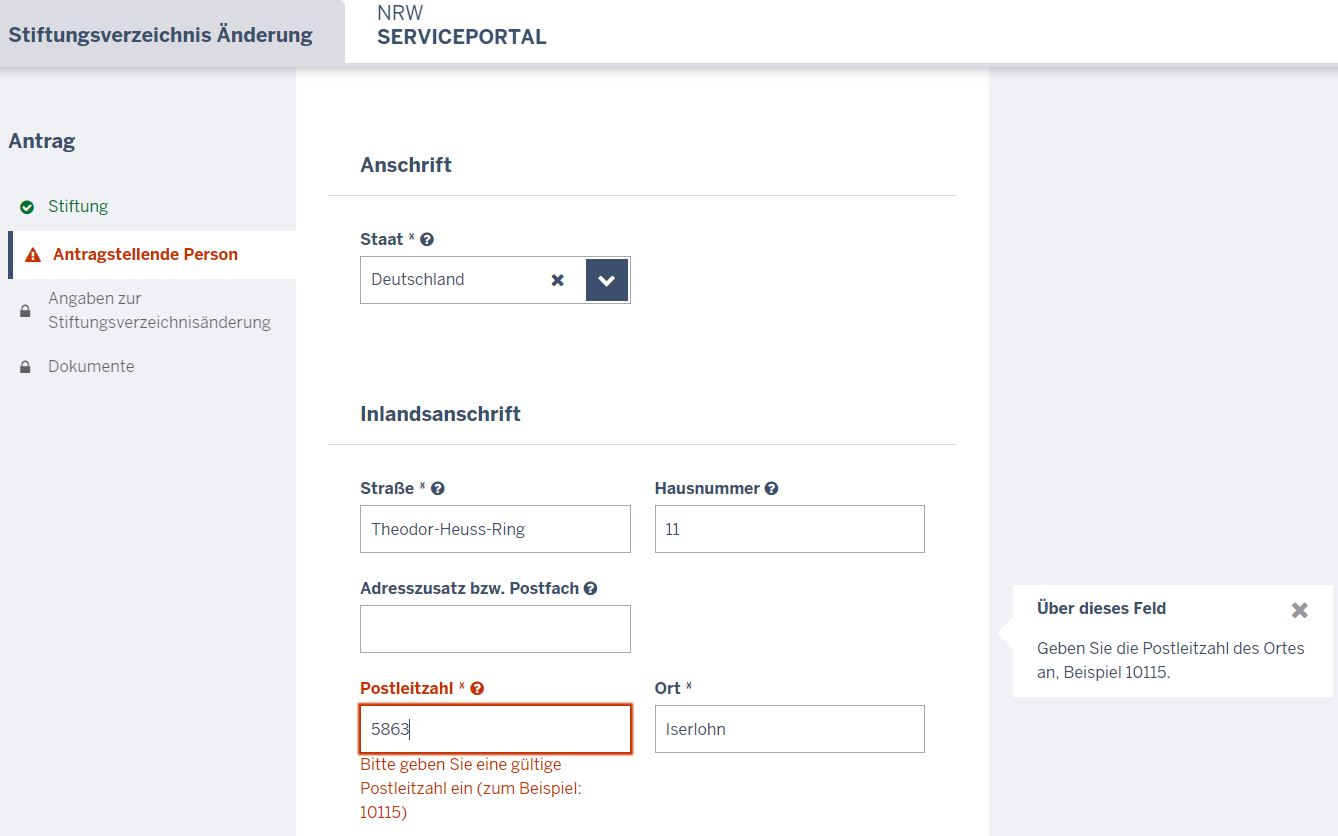
\includegraphics[width=\linewidth]{images/form_adresse.JPG}
  \caption{Ein digitales Formular ``Antrag auf Stiftungsverzeichnis Änderung'', das von der Telekom MMS GmbH modelliert und ins NRW-Serviceportal integriert wurde}
  \label{fig:meineabbildung}
\end{figure}

Um die konkrete Gestaltung und Funktionsweise digitaler Formulare zu veranschaulichen, betrachten wir ein Beispiel (Abb. 2.1). Der Screenshot eines Formularabschnitts aus NRW Serviceportal zeigt typische Merkmale eines digitalen Formulars: eine Navigationsleiste, klar strukturierte und definierte Eingabefelder. Im Gegensatz zu einem Papierformular bietet die digitale Version interaktive Elemente, Dropdown-Menüs für die Auswahl einer Eingabe, Vorbefüllungen persönlicher Daten und Validierungsfunktionen. Hilfetexte und Tooltips sind bereitgestellt, die beim Bedarf den NutzerInnen bei der korrekten Ausfüllung assistieren. Diese Elemente erhöhen nicht nur die Benutzerfreundlichkeit, sondern tragen auch zur Korrektheit und Vollständigkeit der erfassten Daten bei. Der Screenshot stellt somit dar, wie Formulare im eGovernment-Bereich gestaltet sind, um eine effiziente, fehlerfreie und benutzerorientierte Datenerfassung zu ermöglichen. \\

Die Entwicklung und Verwaltung solcher komplexen digitalen Formulare erfordert ein leistungsfähiges Formularmanagementsystem (FMS). Im nächsten Abschnitt wird detailliert erklärt, was ein FMS ausmacht, welche Komponenten zur Verfügung stehen und wie es zur Effizienzsteigerung und Kundenorientierung in der digitalen Verwaltung beiträgt.







% Im Jahre 1450 hat die Geschichte von Formularen mit einem Ablassbrief begonnen. Im Laufe der Zeit hat das Papierformular sein Gestalt immer wieder verändert, von Ablassbrief (1455) über Steuerformulare (1792) und Passagierlisten (1892) bis hin Verwaltungsformulare (1929). Einen digitalen Datenverarbeitungswandel ab der 70er Jahren bezeugte  EDV-Formulare, die viele Vorteile mit sich brachten. Und heute haben wir zwei Begriffe, die die Formularen einen ganz neuen Glanz verleihen : eCommerce und eGovernment. \citep{formulare_schwesinger_2007}\\

% \textbf{Definition: }\textit{``Formulare sind von einer Ordnung bereitgestellte und im Rahmen dieser Ordnung verwaltete Texte mit Lücken, die von individuellen Fällen ausgefüllt werden, die von dieser Ordnung gesucht werden oder diese Ordnung in Anspruch nehmen.'' \cite[S. ~3]{plener_formular_2021}}   \\

% In dieser Arbeit wird über Formulare des eGorvernments gesprochen. Wie in \cite[S.~VI]{plener_formular_2021} gesagt wurde: ``Das Medium \textit{"`Formular"'} transformiert also nicht nur Daten, sondern eine Gestalt von Bürokratie und bürgerlicher Partizipation.'', daher werden auch die Verwaltungdienste in Deutschland kundenorientierter gestaltet und digitalisiert. \\


% Formulare sind Dokumente oder digitale Schnittstellen, die von Bürgern und Unternehmen genutzt werden, um Informationen an die Einrichtungen zu übermitteln. Sie dienen dazu, verschieden Anliegen, Anträge, Meldungen und Informationen zu erfassen und zu verarbeiten. \\